Building on the theoretical framework of Partially Observable Active Markov Games developed in the previous section, we now apply our POLARIS algorithm to concrete social learning scenarios. This implementation demonstrates how our approach bridges theoretical economic models with computational reinforcement learning methods, allowing us to validate theoretical predictions while uncovering new insights about strategic adaptation in partial observability settings.

We implement our Partially Observable Active Markov Game framework to model the two canonical social learning scenarios discussed in the background section: strategic experimentation with observable rewards and learning without experimentation through action observation. By reformulating these economic models as POAMGs, we demonstrate how our framework can capture the sophisticated learning dynamics present in these scenarios while enabling the discovery of complex strategies through our POLARIS algorithm. \footnote{Complete Python implementation is available at \url{https://github.com/ecdogaroglu/POLARIS}.}

\section{Strategic Experimentation}

We reformulate the strategic experimentation model of \citet{keller2020undiscounted} as a Partially Observable Active Markov Game. This framework analyzes undiscounted continuous-time games where a number of symmetric players act non-cooperatively, trying to learn an unknown state of the world governing the risky arm's expected payoff. The state space $S = \{0,1,\ldots,m\}$ represents possible states of the world, with a deterministic transition function since the underlying state remains constant throughout the interaction. Each agent's action space $A^i = [0,1]$ represents the fraction of resources allocated to the risky arm at each decision point, creating a continuous action space that allows for nuanced exploration strategies.

While the original model operates in continuous time with Lévy processes, our POAMG implementation discretizes time using the Euler-Maruyama scheme \citep{kloeden1992numerical, platen1999introduction} for both the background signal and the agents' payoff processes. This numerical method is widely used for approximating solutions to stochastic differential equations driven by both Brownian motion and Poisson processes.

The agents receive a public signal produced by the background process, which leads to the observation function:

\begin{equation}
    O^i(s, o) = \mathbb{P}(o_t | B_{t-1:t})
\end{equation}

where $o_t$ represents the observation at discrete time step $t$ and $B_{t-1:t}$ represents the signal increment in discrete time. To address the time-dependent nature of Lévy processes while maintaining compatibility with our POAMG framework, we formulate the reward function for each agent $i$ as:

\begin{equation}
    R^i(s, a^i) = (1-a^i)r_\textit{safe} + a^i \frac{X^i_{t-1:t}}{\Delta t}
\end{equation}
where $\Delta t$ is the discretization time step,
\begin{equation}
    X^i_{t-1:t} = \alpha_s \Delta t + \sigma (W^i_t - W^i_{t-1}) + \Delta Y^i_t,
\end{equation}
$(W^i_t - W^i_{t-1}) \sim \mathcal{N}(0, \Delta t)$, and $\Delta Y^i_t$ is the increment of the compound Poisson processes over the interval $[t-1, t]$.
This normalization converts accumulated rewards to instantaneous reward rates, preserving the incentive structure of the original model. A comprehensive mathematical treatment of this discretization approach, including convergence properties and the preservation of strategic incentives, is provided in Appendix \ref{appendix:levy_discretization}.

Each agent observes the increments in the public background signal, their own payoff process (dependent on their allocation $a^i$ to the risky arm and the true state $\omega$), and the allocations together with the rewards of all other agents. The unique feature of the strategic experimentation model is the explicit form of the symmetric Markov perfect equilibrium, which depends only on three factors: the safe payoff, the expected current payoff of the risky arm, and the expected full-information payoff. To validate this theoretical result, we configure POLARIS to measure: (1) The cutoff belief at which agents switch between the safe and risky arm
(2) The relationship between individual experimentation intensity and group experimentation intensity
(3) Free-riding behavior as a function of the number of players
(4) Strategy independence from the specific payoff-generating process
\iffalse
    For experimental validation, we implement three distinct payoff-generating processes that preserve the same reward statistics: pure Brownian motion with unknown drift, pure Poisson processes with unknown intensity, and mixed Lévy processes with both continuous and jump components. In all three cases, the theory predicts identical equilibrium strategies when expressed in terms of the incentive to experiment $I(\pi) = \frac{f(\pi)-s}{s-m(\pi)}$ when $m(\pi) < s$, and $I(\pi) = \infty$ otherwise, where $\pi$ represents the belief state.
\fi
To measure convergence to equilibrium behavior, we track the Kullback-Leibler divergence (KL divergence) between agents' actual strategies and the theoretically optimal strategy specified in Keller and Rady's work. The KL divergence is calculated as

\begin{equation}
    D_{KL}(P||Q) = \sum_{x} P(x) \log\frac{P(x)}{Q(x)},
\end{equation}

where $P$ represents the agent's learned policy distribution and $Q$ represents the theoretical optimal policy distribution at each belief state:

\begin{equation}
    a^*(b) =
    \begin{cases}
        0                    & \text{if } I(b) \leq k_0,            \\
        \frac{I(b)-k_0}{n-1} & \text{if } k_0 < I(b) < k_0 + n - 1, \\
        1                    & \text{if } I(b) \geq k_0 + n - 1.
    \end{cases}
\end{equation}

\iffalse
    We also assess the rate of social learning by measuring the expected time until agents' posterior beliefs concentrate within an $\epsilon$-neighborhood of the true state. The background information in this model ensures exponentially fast convergence, which is empirically validated by fitting an exponential decay curve to the mean distance between current beliefs and true state across multiple simulation runs.
\fi
For varying group sizes $n \in \{2,4,8,16\}$, we measure the relationship between individual and group experimentation. The theory predicts that the set of beliefs for which no experimentation occurs remains unchanged as $n$ increases—a stark manifestation of free-riding behavior. Additionally, the theory predicts that in regions of partial experimentation, the intensity per agent will decrease with $n$, while the total group intensity increases. These predictions create testable patterns that our POLARIS implementation can validate.
\iffalse
    An important methodological insight from this implementation is the impact of the background signal $k_0$ on learning dynamics. As $k_0$ approaches zero, the equilibrium strategy converges monotonically to a well-defined limit. However, without background information, the strong long-run average criterion would yield an expectation of minus infinity, making the framework inapplicable. We thus implement a parametric analysis with diminishing values of $k_0$ to approximate the limit behavior predicted by the theory.
\fi

\begin{figure}[!htbp]
    \centering
    \begin{minipage}[t]{0.48\textwidth}
        \centering
        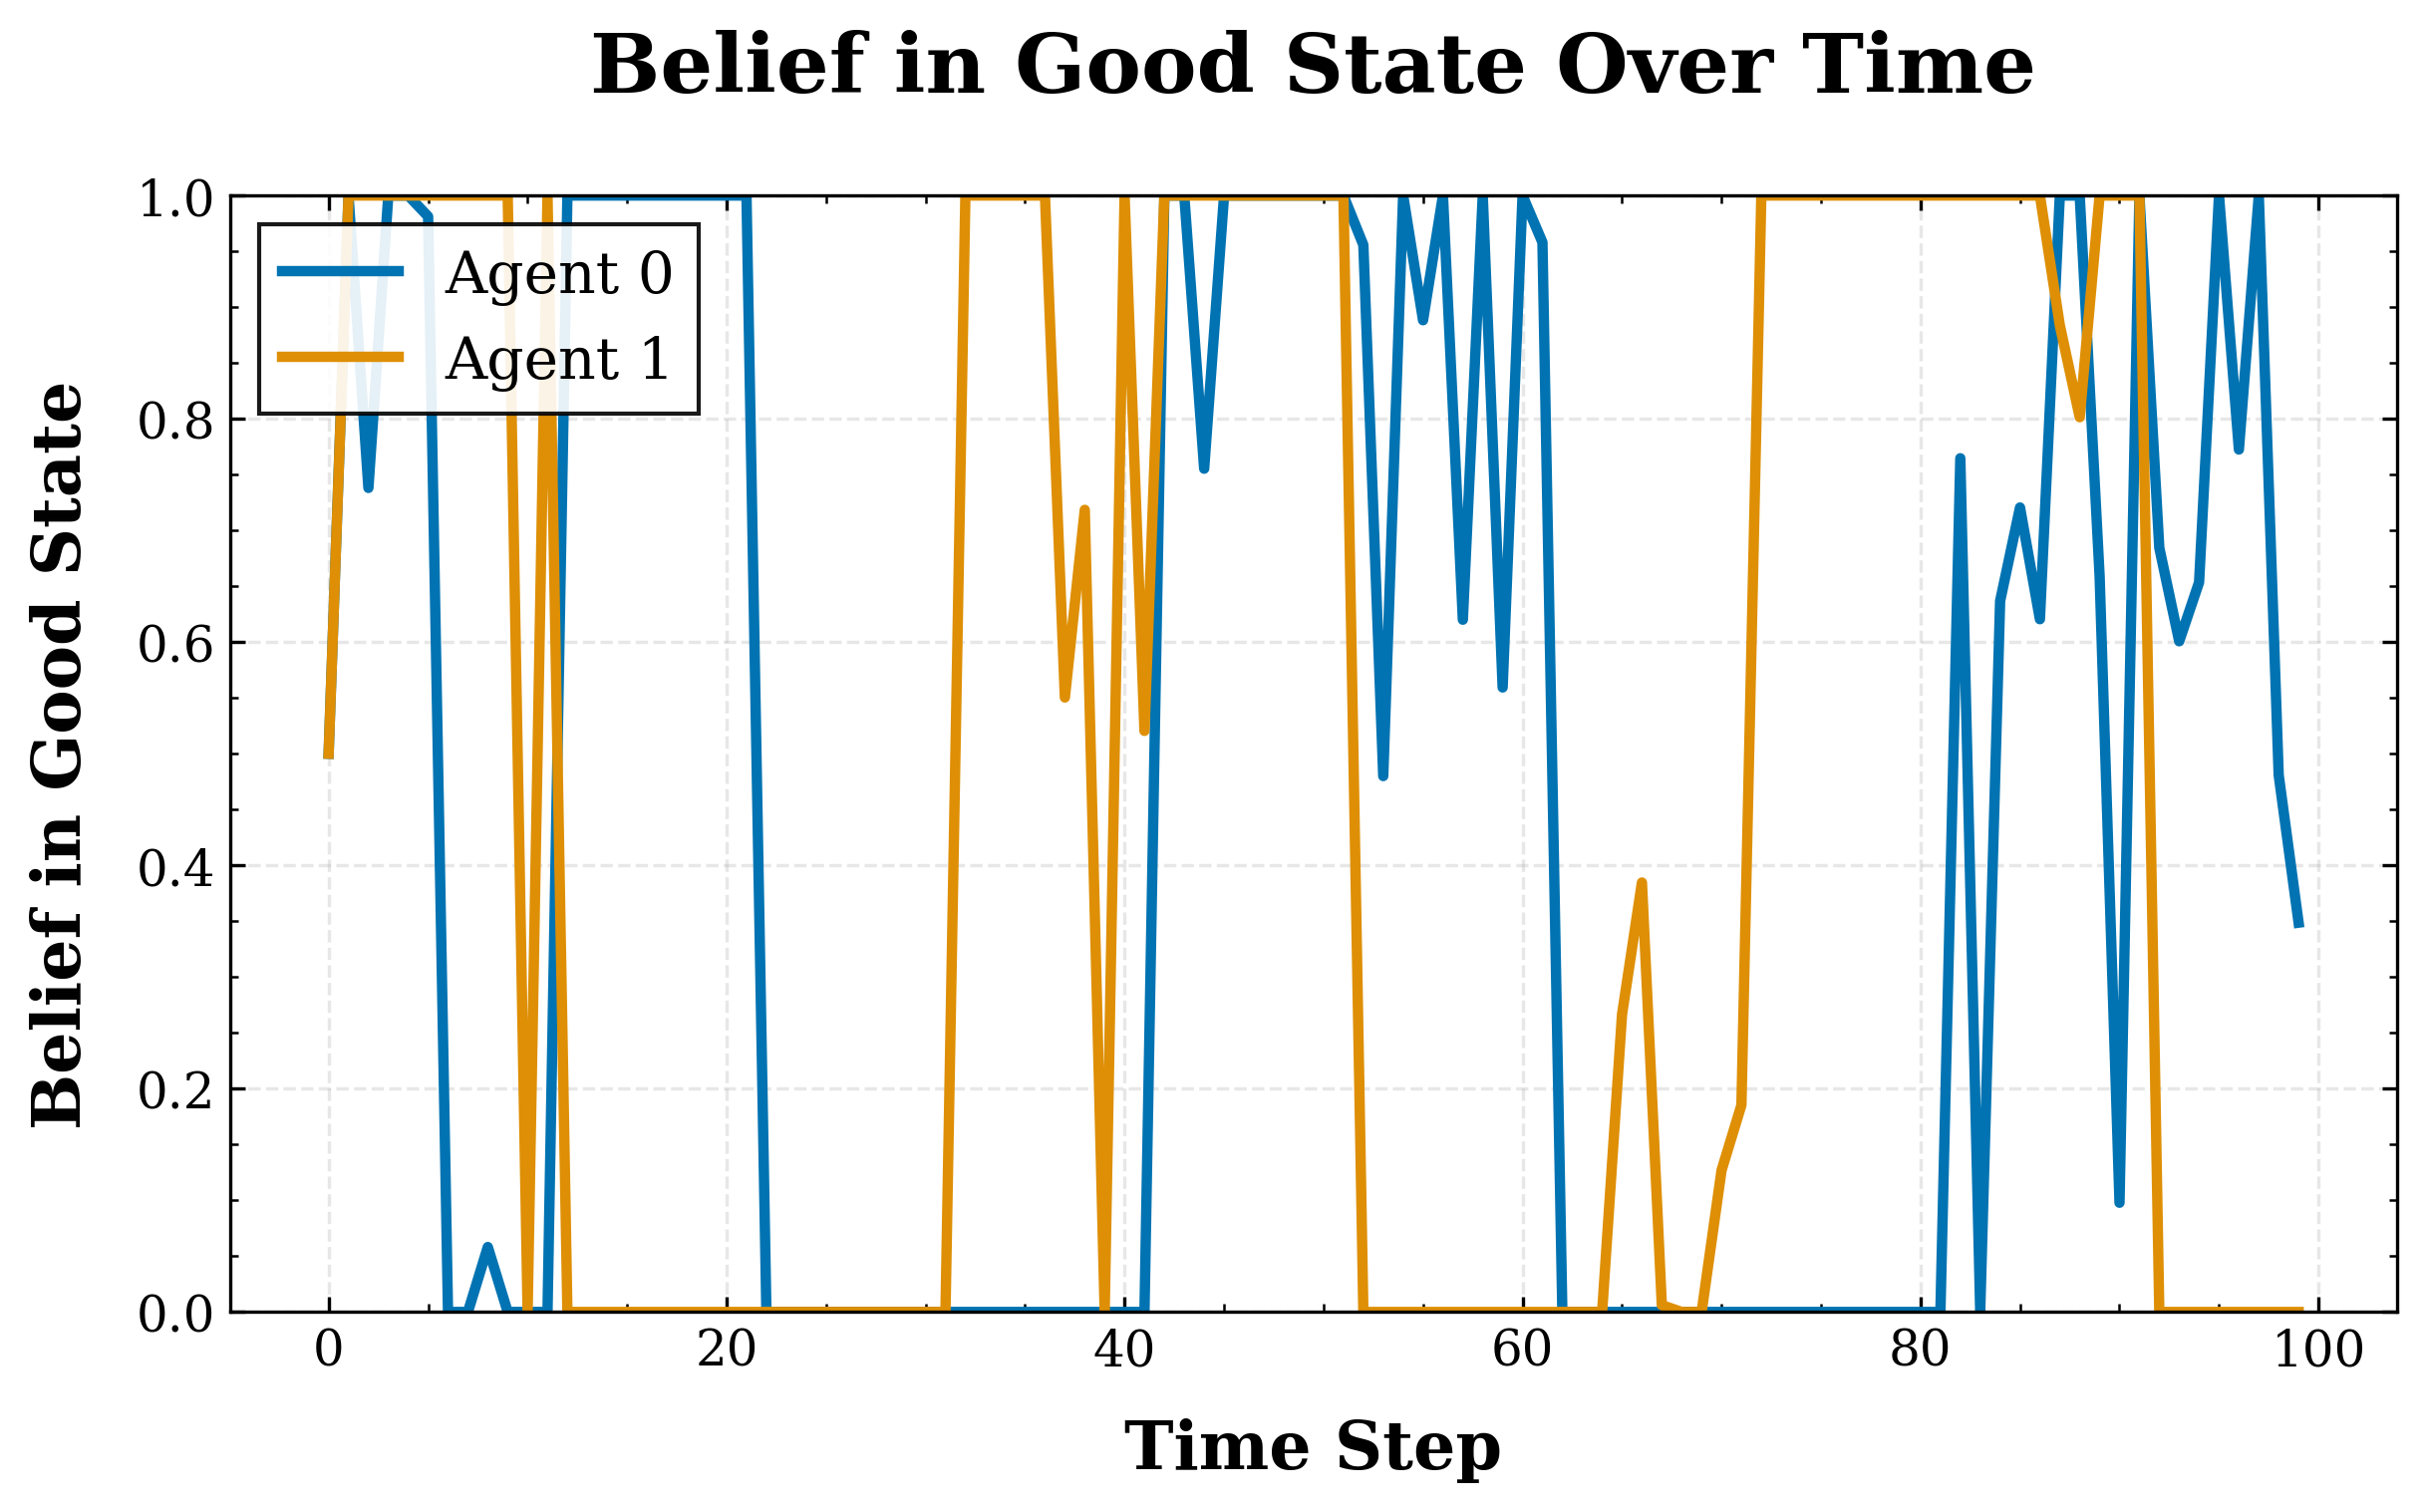
\includegraphics[width=\textwidth]{../code/polaris/results/strategic_experimentation_agents_2_gnn/network_complete_agents_2/good_belief_over_time.png}
        \subcaption{Good state beliefs over time, demonstrating convergence to the true state.}
        \label{fig:good_belief_over_time}
    \end{minipage}
    \hfill
    \begin{minipage}[t]{0.48\textwidth}
        \centering
        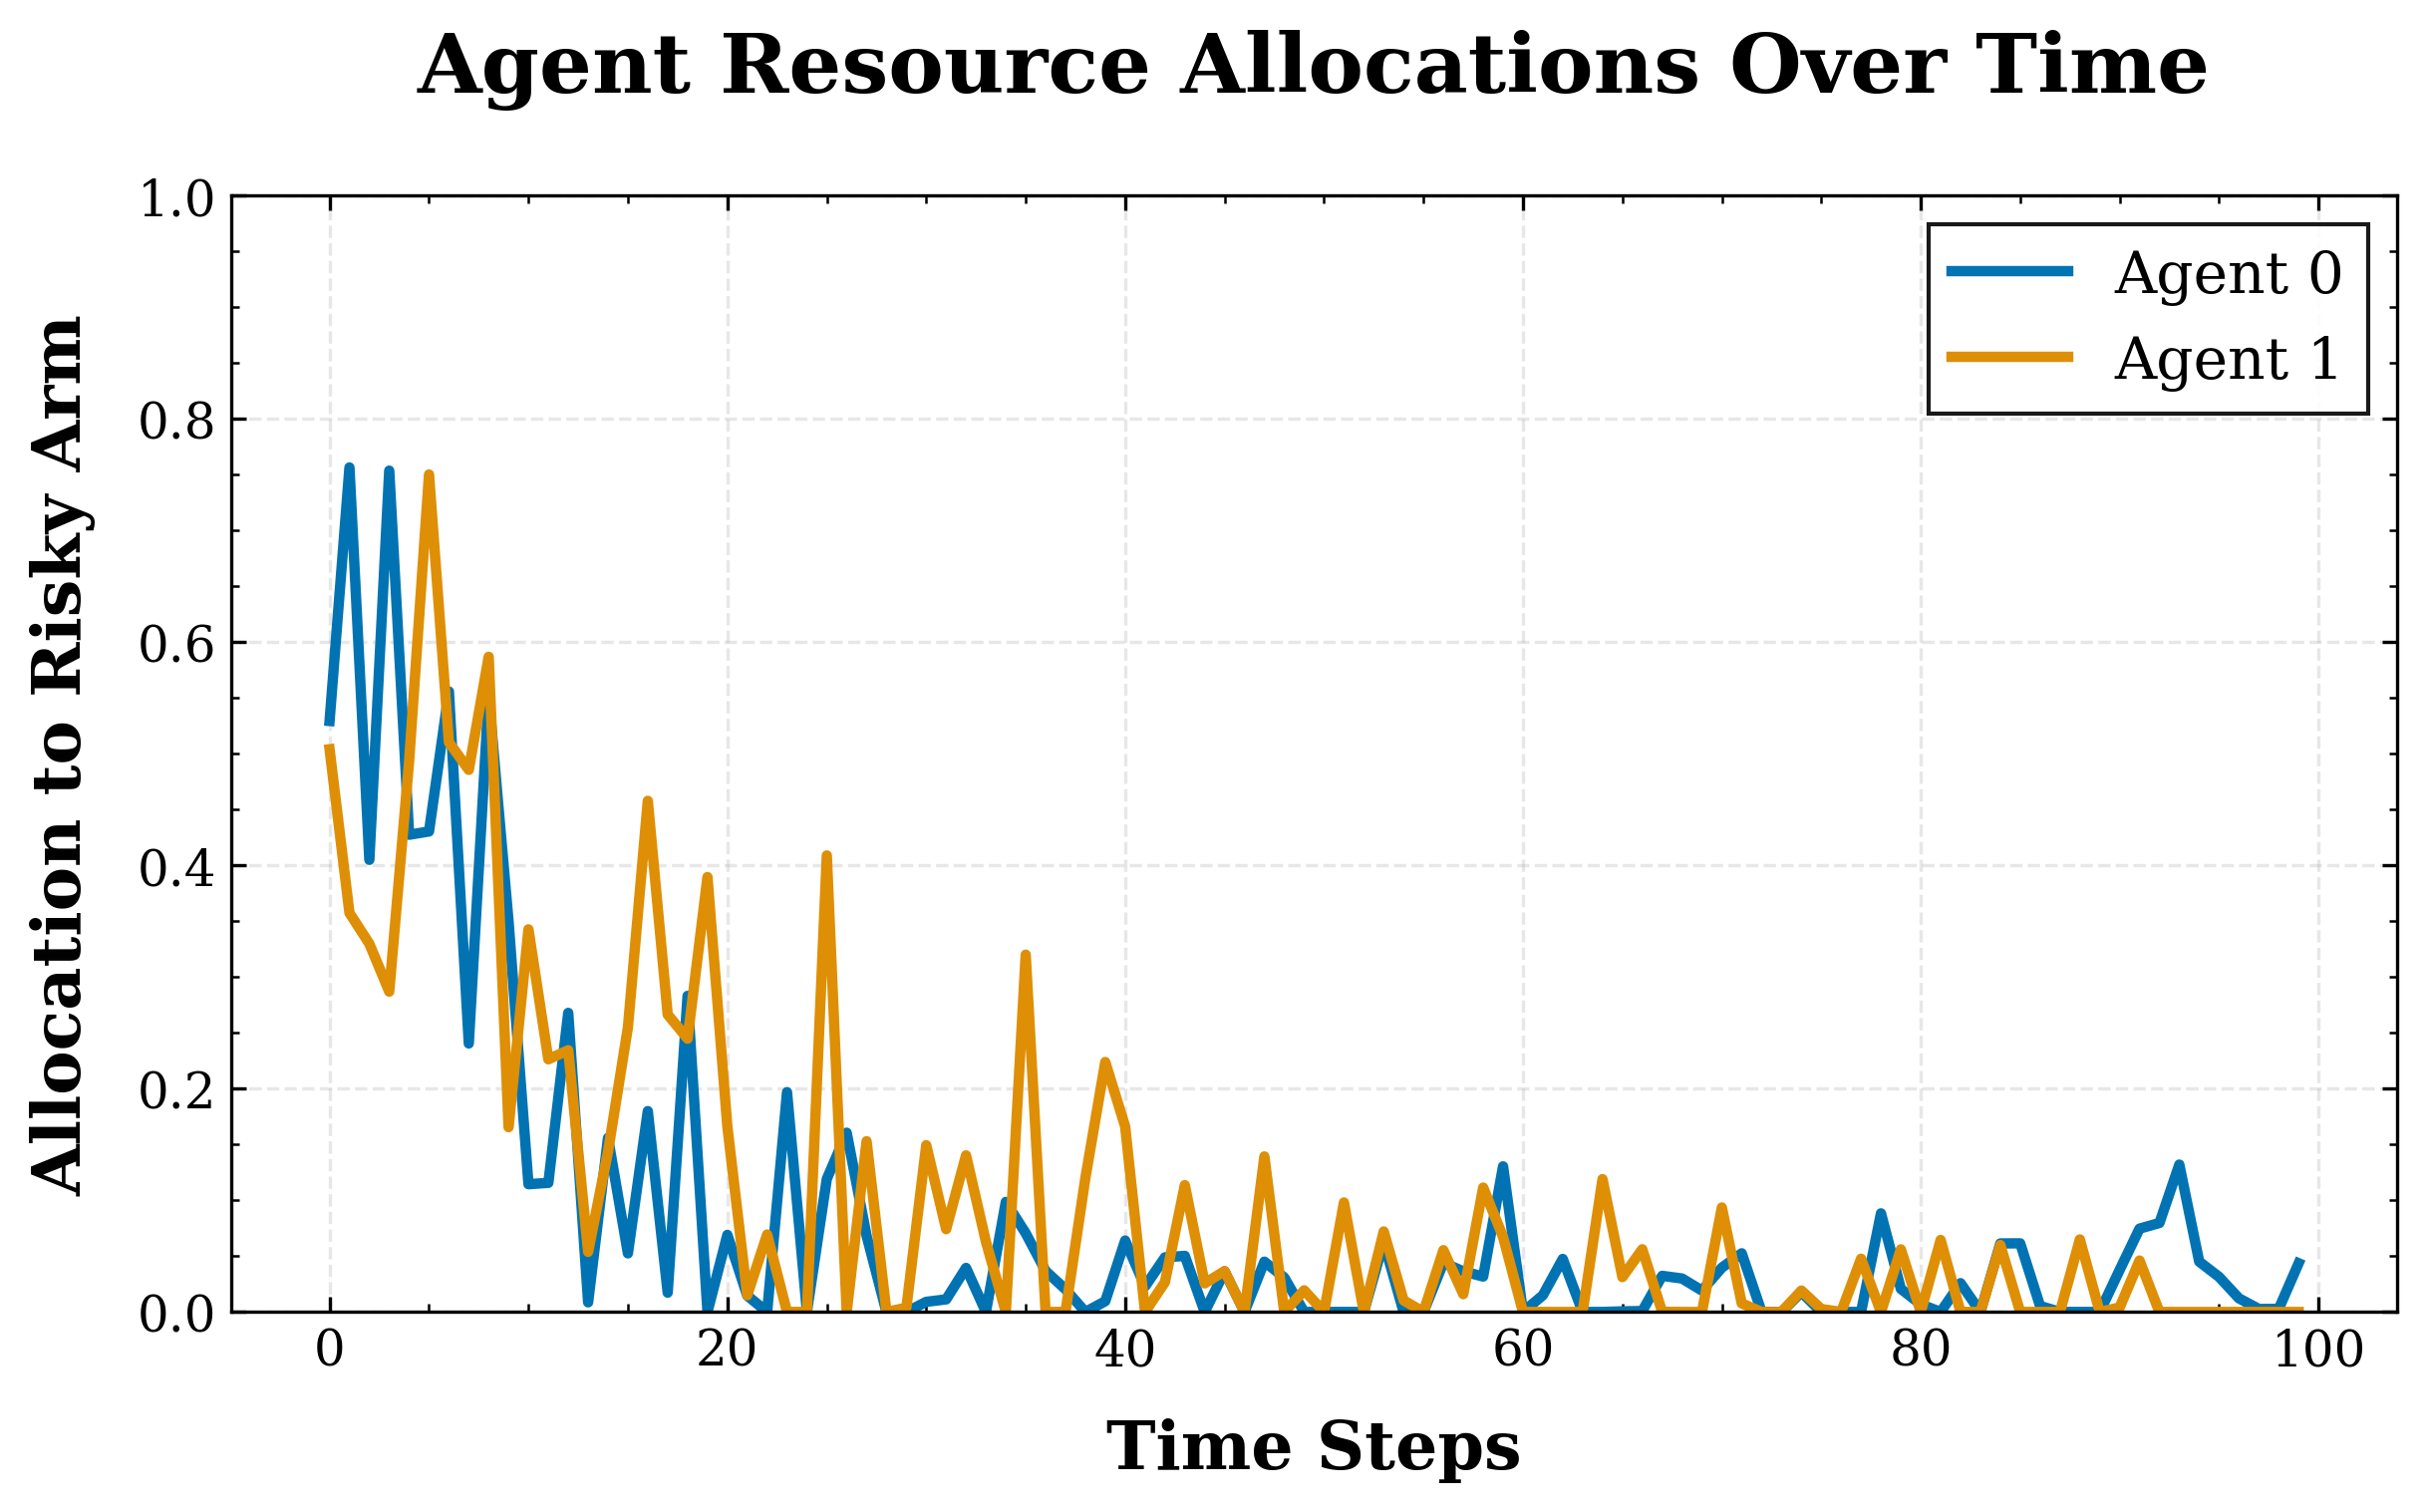
\includegraphics[width=\textwidth]{../code/polaris/results/strategic_experimentation_agents_2_gnn/network_complete_agents_2/agent_allocations.png}
        \subcaption{Agent allocations over time, demonstrating eventual adoption of the best strategy.}
        \label{fig:agent_allocations}
    \end{minipage}
    
    \vspace{0.3cm}
    
    \begin{minipage}[t]{0.48\textwidth}
        \centering
        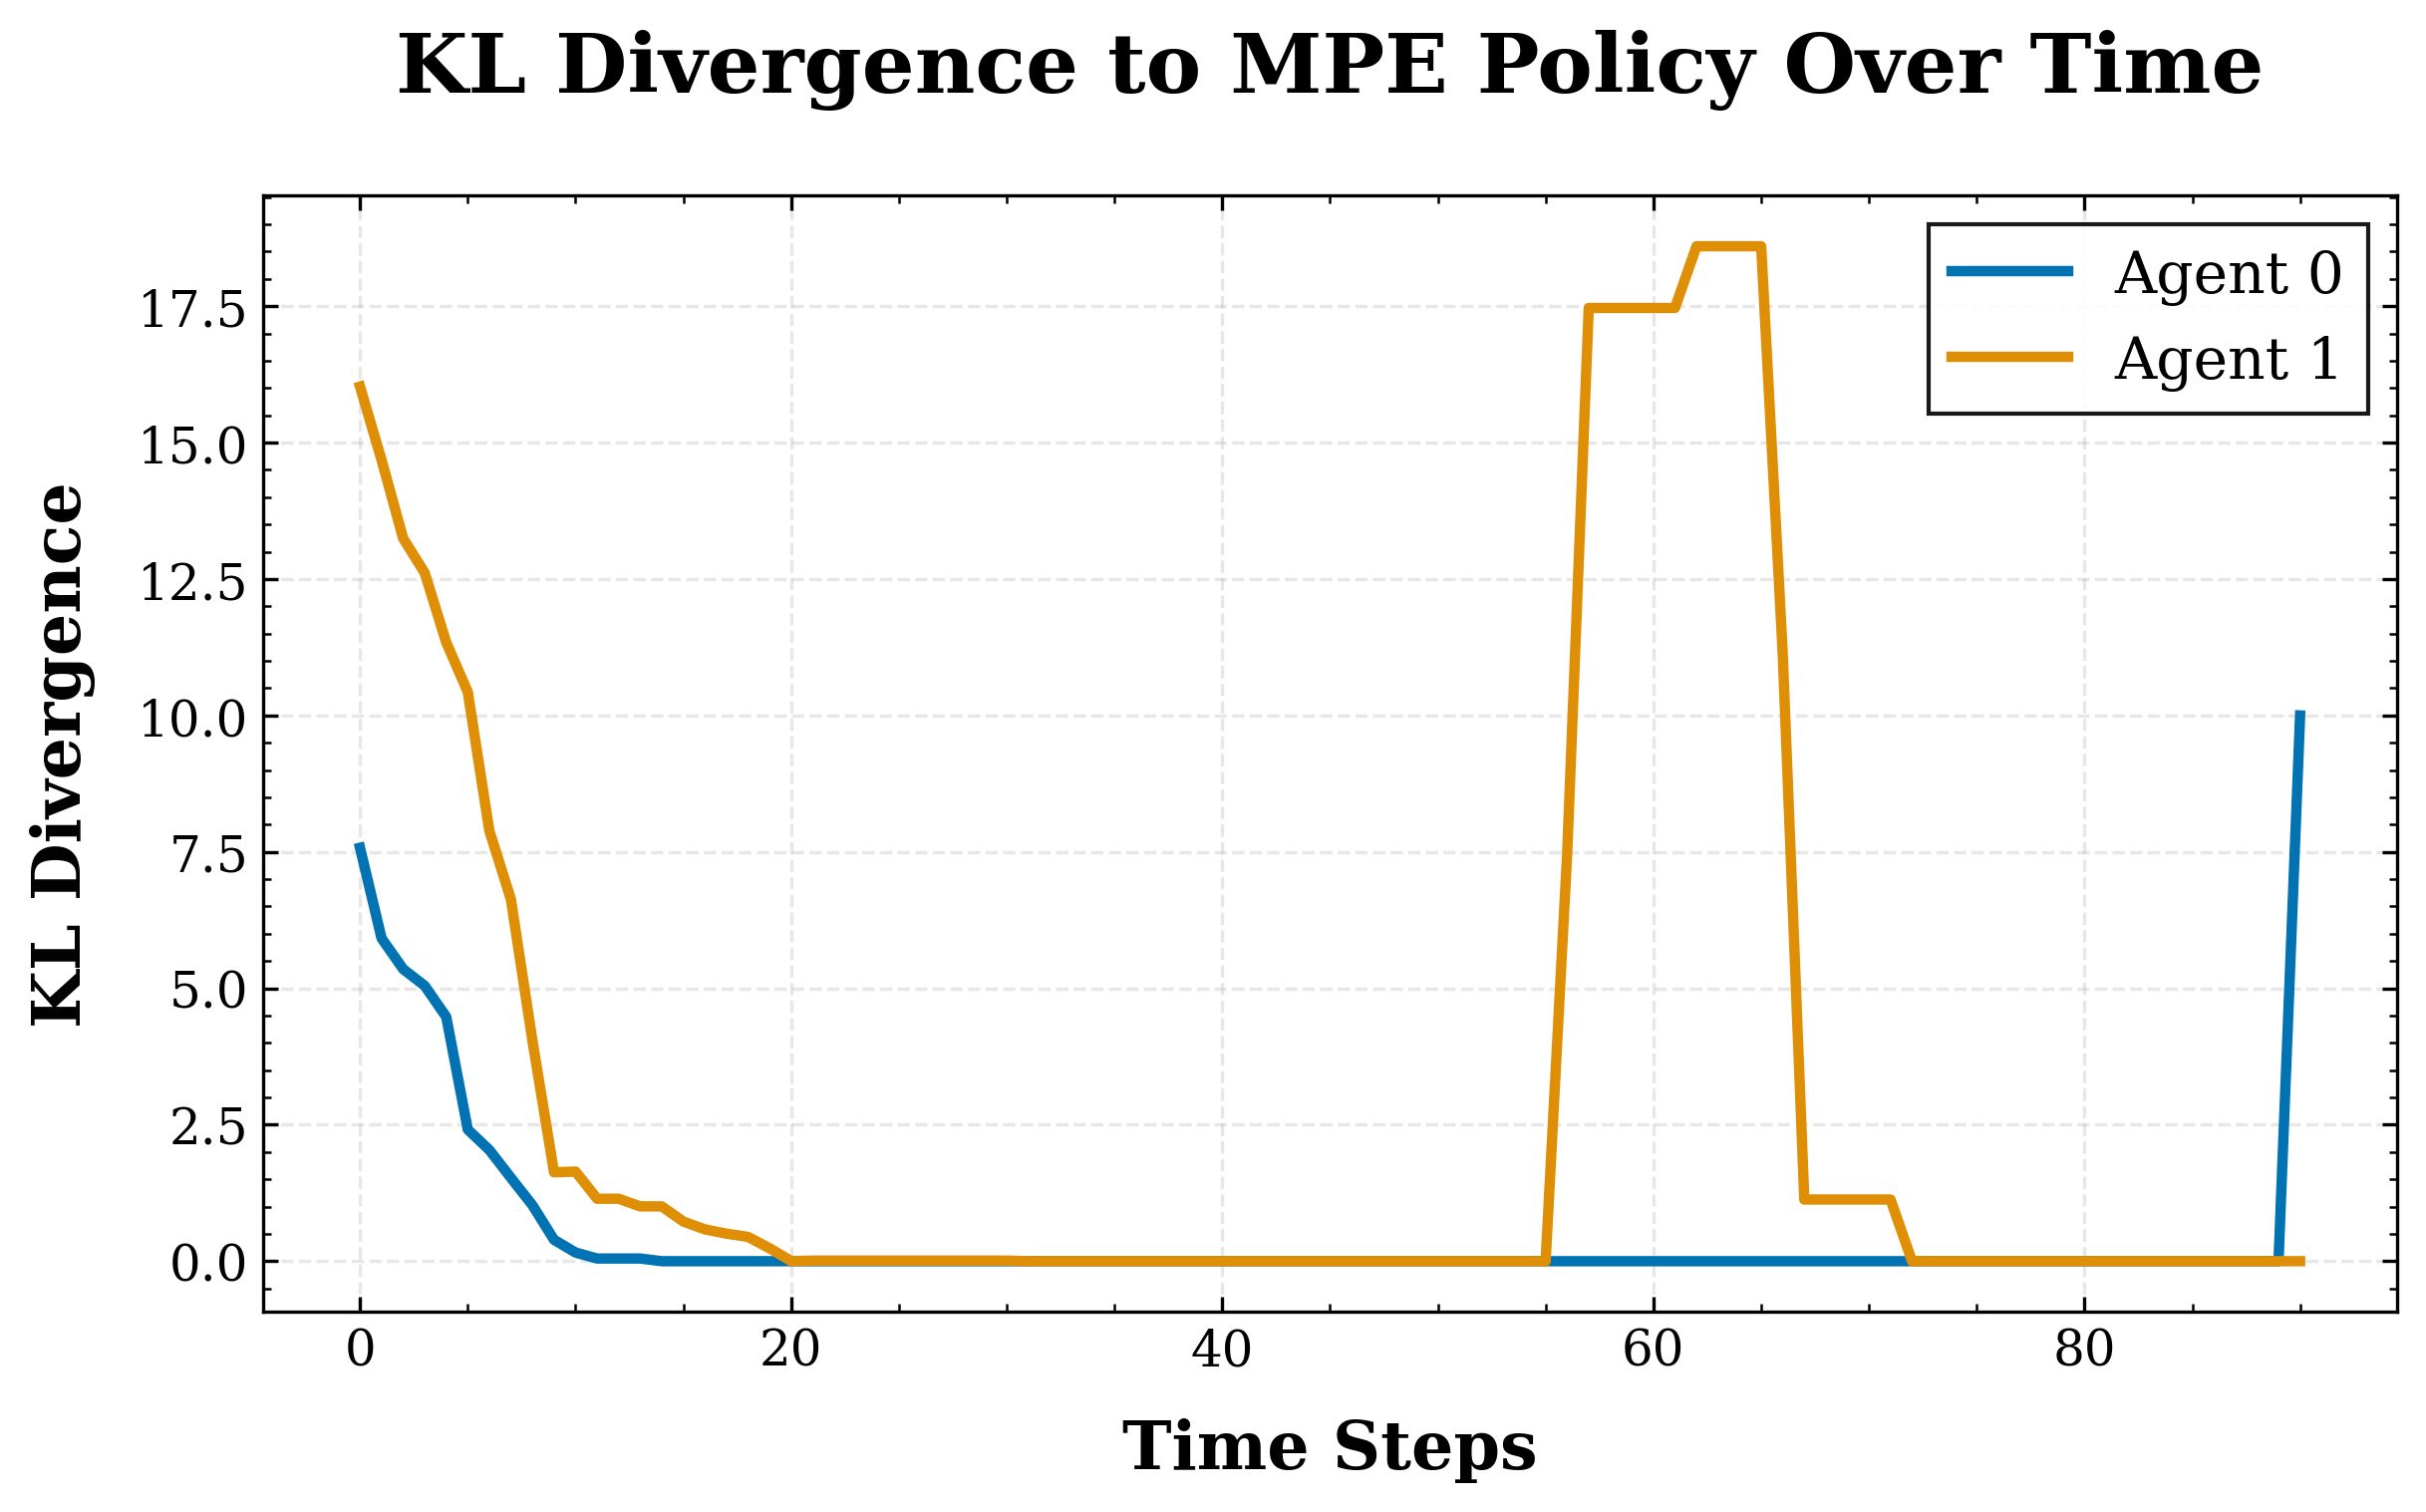
\includegraphics[width=\textwidth]{../code/polaris/results/strategic_experimentation_agents_2_gnn/network_complete_agents_2/kl_divergence.png}
        \subcaption{KL divergence between agents' learned strategies and the theoretical optimal strategy as a function of time, demonstrating convergence to equilibrium behavior.}
        \label{fig:kl_divergence}
    \end{minipage}
    \hfill
    \begin{minipage}[t]{0.48\textwidth}
        \centering
        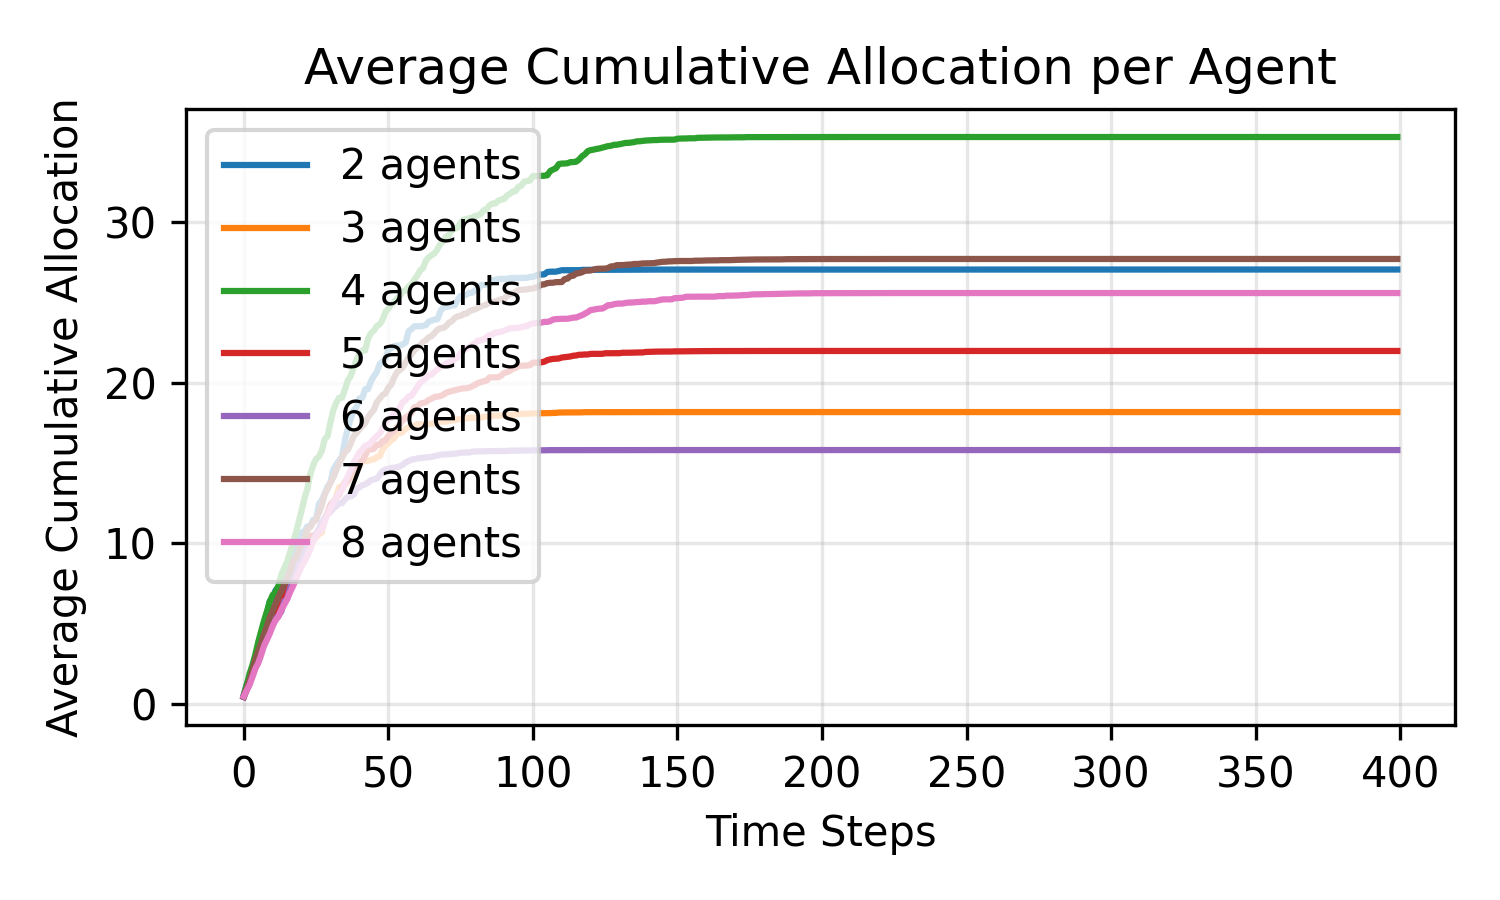
\includegraphics[width=\textwidth]{../code/polaris/results/strategic_experimentation/sweep_allocations/average_cumulative_allocation_per_agent_over_time.png}
        \subcaption{Average cumulative allocation per agent over time across different network configurations, demonstrating independence from the network size.}
        \label{fig:average_cumulative_allocation_per_agent_over_time}
    \end{minipage}
    
    \caption{Learning dynamics in the strategic experimentation model}
    \label{fig:strategic_experimentation_results}
\end{figure}


Our experimental results confirm that POLARIS agents converge to the theoretically predicted equilibrium regardless of the specific payoff-generating process employed. This validation demonstrates the framework's ability to capture the sophisticated strategic considerations of undiscounted multi-agent learning, providing computational support for the theoretical predictions of Keller and Rady. Furthermore, our results show that the mixed Lévy process case—not analytically tractable in the original paper due to its complexity—exhibits the same qualitative behavior as the pure Brownian and Poisson cases, providing evidence for the robustness of the theoretical framework.

\section{Learning Without Experimentation}

We reformulate the learning without experimentation model of \citet{brandl2024} as a Partially Observable Active Markov Game. In this formulation, the state space $S = \{s^1, s^2, \ldots, s^m\}$ represents possible states of the world, with a deterministic transition function since the state remains constant. Each agent's action space $A^i = \{a^1, a^2, \ldots, a^m\}$ corresponds to potential states, where $a^j$ is the unique optimal action is state $s^j$. In addition to observing their neighbors' actions, each agent receives a private signal $o^i_t \in \Omega^i = S$ drawn from distribution:

\begin{equation*}
    O^i(s,o) =
    \begin{cases}
        q               & \text{if } s = o \\
        \frac{1-q}{m-1} & \text{otherwise}
    \end{cases}
\end{equation*}
where $q > 1/m$ is the signal accuracy. Since agents don't observe real rewards in this model, we construct an observed reward function that facilitates learning:

\begin{equation*}
    R^i(s_t, a^i_t) = v(o^i_t, a^i_t) = \frac{q \cdot \mathbb{I}_{\{a^i_t = \varphi(o^i_t)\}} - (1 - q) \cdot \mathbb{I}_{\{a^i_t \neq \varphi(o^i_t)\}}}{2q - 1}
\end{equation*}

where $\varphi$ maps states to their corresponding correct actions. \footnote{Formally, the mapping $\varphi: S \rightarrow A$ is a bijective function defined as $\varphi(s^j) = a^j$ for all $j \in \{1,2,...,m\}$, associating each state with the action having the same index.} This construction ensures the expected reward matches the true utility function in expectation: \footnote{See \ref{appendix:observed_reward_derivation} for a detailed derivation and the formulation for a generic dimension $m$.}

\begin{equation*}
    \mathbb{E}_{o \sim \mu^{s}}[v(o, a)] = u(s, a) = \mathbb{I}_{\{a = \varphi(s)\}}.
\end{equation*}


This construction ensures agents are rewarded based on their posterior belief given the private signal, maintaining compatibility with the original model's incentive structure while providing a learning signal for POLARIS.

\subsection{Experimental Setup}

We implement comprehensive experiments to validate these theoretical predictions and explore the learning dynamics under various network structures. Our experimental protocol examines network sizes of $n \in \{1, 2, 4, 8\}$ agents; network topologies including complete, ring, star, and random networks; signal accuracy of $p = 0.75$ (matching the paper's example where $r_{\text{aut}} = 0.14$, $r_{\text{crd}} = 0.55$, and $r_{\text{bdd}} = 1.10$); and learning metrics consisting of empirical learning rates extracted via log-linear regression.

For each configuration, we run multiple independent episodes with randomly initialized true states and agents. Our analysis follows a two-stage approach. First, for each episode $k$, we track each agent's incorrect action probability over time: 
\begin{equation}
    \hat{P}_{t,k}^i = 1 - \pi_t^i(a_{\omega_k} | b^i_t, z^i_t)
\end{equation}

And estimate individual learning rates by fitting: 
\begin{equation}
    \log \hat{P}_{t,k}^i \approx -r_k^i t + c_k^i
\end{equation}

To identify the fastest and slowest learners for that episode: 
\begin{equation}
    i_{\text{fast}}^k = \arg\max_i r_k^i
\end{equation} 
 \begin{equation}
    i_{\text{slow}}^k = \arg\min_i r_k^i
\end{equation}

Second, we aggregate the performance of fastest and slowest learners across episodes:

\begin{equation}
    \bar{P}_t^{\text{fast}} = \frac{1}{N_{\text{episodes}}} \sum_{k=1}^{N_{\text{episodes}}} \hat{P}_{t,k}^{i_{\text{fast}}^k}
\end{equation}
\begin{equation}
    \bar{P}_t^{\text{slow}} = \frac{1}{N_{\text{episodes}}} \sum_{k=1}^{N_{\text{episodes}}} \hat{P}_{t,k}^{i_{\text{slow}}^k}
\end{equation}

where $N_{\text{episodes}}$ is the number of episodes. This methodology allows us to examine the distribution of learning rates that emerge from the same network structure across different realizations, revealing whether the theoretical bounds hold regardless of which specific agent becomes the fastest or slowest learner in any given episode.

\subsection{Results and Analysis}

Our experimental results provide strong validation of the theoretical predictions while revealing additional insights into the learning dynamics. We begin by addressing a key methodological consideration before examining our main findings.

\paragraph{Methodological Context} The theoretical autarky rate of $r_{\text{aut}} \approx 0.14$ (derived using large deviation theory for random walks) differs substantially from the empirical single-agent POLARIS performance of approximately $0.35$ (Figure \ref{fig:size_comparison}). This difference reflects fundamental methodological distinctions: the theoretical analysis assumes agents follow the maximum likelihood strategy with perfect signal processing, while POLARIS agents learn policies through reinforcement learning with our constructed reward function and Transformer-based processing. Additionally, the theoretical rate derives from asymptotic analysis as $t \to \infty$, whereas our empirical measurements occur over finite horizons. Despite these methodological differences, both approaches provide complementary insights into learning performance bounds and achievable rates in practice.

\begin{figure}[!htbp]
    \centering
    \includegraphics[width=\textwidth]{../code/polaris/results/brandl_experiment/agent_performance/fastest_slowest_network_sizes_evolution.png}
    \caption{Fastest vs slowest agent learning trajectories across network sizes. Each subplot shows the mean incorrect action probability over time with $95\%$ confidence intervals (shaded regions) for the fastest (green) and slowest (red) learning agents. The learning rates $r$ are calculated using log-linear regression. Results demonstrate the learning barrier effect where slowest agents remain bounded while fastest agents achieve superior performance in larger networks.}
    \label{fig:size_comparison}
\end{figure}

Our analysis reveals three key phenomena that validate and extend the theoretical predictions: the emergence of learning barriers, the realization of coordination benefits, and the dynamic formation of information revelation roles.

\paragraph{Learning Barriers Emerge Systematically} Across all network configurations and episodes, we consistently observe a significant reduction in the slowest-learning agent's rate compared to the autarky rate. Figure \ref{fig:size_comparison} demonstrates this barrier effect by aggregating the trajectories of whichever agent learns slowest in each episode. This finding directly supports the theoretical prediction of Theorem 1. While we cannot observe whether the bound significantly exceeds the autarky rate as the theorem suggests—such validation would require much larger networks and higher computational resources—the consistent emergence of learning barriers across all configurations provides strong empirical support for the theoretical framework.

\paragraph{Coordination Benefits Materialize in Larger Networks} In networks with $n \geq 4$ agents, the fastest-learning agents consistently demonstrate superior performance compared to isolated agents, confirming the coordination benefits predicted by Theorem 2. This demonstrates that social learning enables some agents to surpass single-agent performance, though at the expense of others. The systematic nature of this improvement across different network sizes suggests that the coordination benefits are robust features of multi-agent social learning rather than artifacts of specific configurations. However, similar to our findings on learning barriers, we cannot observe whether the learning rate of the slowest-learning agent can surpass the autarky rate for sufficiently large networks as the theorem suggests.

\paragraph{Information Revelation Through Dynamic Role Assignment} Our results reveal a systematic pattern where agents naturally emerge as either information generators or information exploiters within each episode. The agents that learn slowest exhibit higher variance in their action choices (evident from the wider confidence intervals in Figure \ref{fig:size_comparison}), indicating more exploratory behavior that enables other agents to make better-informed decisions. Crucially, this division of labor emerges dynamically—different agents assume these roles across episodes, suggesting the phenomenon arises from learning dynamics rather than fixed agent characteristics.

\begin{figure}[!htbp]
    \centering
    \includegraphics[width=\textwidth]{../code/polaris/results/brandl_experiment/agent_performance/fastest_slowest_network_types_evolution.png}
    \caption{Fastest vs slowest agent learning trajectories across network topologies. Each subplot compares performance in different network structures (complete, ring, star, random) with 4 agents. The confidence intervals reveal how network topology affects the learning rate disparity between fastest and slowest agents, with complete networks showing the most pronounced differentiation due to enhanced information sharing.}
    \label{fig:type_comparison}
\end{figure}

\paragraph{Network Structure Shapes Information Flow} Figure \ref{fig:type_comparison} reveals how network topology influences learning dynamics. Complete networks facilitate the most effective information sharing, producing the largest performance gaps between fastest and slowest learners. Ring networks show more uniform learning rates due to limited information flow, while star networks create pronounced differences between central and peripheral agents. These patterns align with theoretical insights that information aggregation depends critically on network structure, though the specific mechanisms through which topology affects learning warrant further investigation.

To understand the underlying mechanisms determining which agents become information generators, we examine the roles of network position and signal quality—two factors that could potentially explain the emergence of learning disparities.

\begin{figure}[!htbp]
    \centering
    \includegraphics[width=\textwidth]{../code/polaris/results/brandl_experiment/agent_performance/slowest_agent_network_positions.png}
    \caption{The position of the slowest-learning agent in the network over time. The frequency of being the slowest-learning agent is calculated as the average number of episodes that this position is occupied by the slowest-learning agent. The slowest-learning agent is the agent that learns the slowest in each episode.}
    \label{fig:slowest_agent_network_positions}
\end{figure}

\paragraph{Signal Quality, Not Network Position, Determines Learning Roles} Our analysis reveals that network position alone cannot predict learning performance. Figure \ref{fig:slowest_agent_network_positions} shows that the identity of the slowest-learning agent distributes approximately uniformly across network positions, indicating that structural network advantages do not systematically determine learning performance. This finding suggests that network topology alone cannot predict which agents will act as information generators.

\begin{figure}[!htbp]
    \centering
    \includegraphics[width=\textwidth]{../code/polaris/results/brandl_experiment/agent_performance/signal_quality_vs_learning_performance.png}
    \caption{The learning performance of POLARIS agents as a function of the signal quality. Each point corresponds to a single agent in a single episode. The signal quality is calculated as the average correctness of the private signal within the episode.}
    \label{fig:signal_quality_vs_learning_performance}
\end{figure}

In contrast, Figure \ref{fig:signal_quality_vs_learning_performance} demonstrates a strong positive correlation between signal quality and learning performance. Agents who receive lower-quality private signals consistently exhibit slower learning rates, indicating that the primary determinant of becoming a slow learner is the stochastic realization of signal quality rather than strategic positioning within the network. Agents receiving more accurate private signals naturally learn faster, while those receiving noisier signals become information generators whose exploratory behavior, though individually costly, benefits the overall network through enhanced information revelation.

\paragraph{Implications and Validation} These results demonstrate that our POAMG framework successfully captures the essential features of social learning without experimentation, validating both the learning barriers that limit information aggregation and the coordination benefits that emerge in well-connected networks. The computational approach complements theoretical analysis by revealing the dynamics of strategy discovery and the distributional properties of learning rates across different network configurations.

Crucially, our episode-wise analysis methodology shows that the theoretical bounds from \citet{brandl2024} represent robust properties of the multi-agent learning system rather than characteristics of specific agents. In any given episode, different agents may assume the roles of fastest or slowest learners, yet the aggregate behavior consistently respects the theoretical limits. This emergent division of labor—where some agents naturally become information generators while others exploit this information—arises from the learning dynamics themselves rather than from predetermined agent roles, providing computational validation for the theoretical insights about social learning barriers and coordination benefits.


